\section{Results Under Strict Protocols}
\label{sec:results}

Every method in this section is trained and evaluated on the identical
committed splits, with the same optimiser, epoch budget, class weighting and
early-stopping rule where those apply. Deviations from each baseline's original
configuration are recorded in the artifact and in the result files themselves,
never left unstated.

% Generated by scripts/make_paper_assets.py. Do not edit by hand.
\begin{table}[t]
\centering
\small
\begin{tabular}{lccc}
\toprule
Method & Macro-F1 & Balanced acc. & Params \\
\midrule
Majority class & 0.006 & 0.056 & --- \\
\midrule
\multicolumn{4}{l}{\emph{Identifier shortcuts}} \\
Destination port only & \textsc{todo} & \textsc{todo} & --- \\
SNI string only & 0.967 & 0.968 & --- \\
Server IP / prefix only & 0.768 & 0.769 & --- \\
Server AS only & 0.162 & 0.229 & --- \\
Transport protocol only & \textsc{todo} & \textsc{todo} & --- \\
\midrule
\multicolumn{4}{l}{\emph{Classical statistical}} \\
5 flow statistics (RF) & 0.415 & 0.421 & --- \\
Packet-size histogram (XGB) & 0.713 & 0.719 & --- \\
CUMUL & 0.373 & 0.402 & --- \\
AppScanner & 0.772 & 0.775 & --- \\
$k$-fingerprinting & 0.590 & 0.597 & --- \\
\midrule
\multicolumn{4}{l}{\emph{Deep, non-pretrained}} \\
DeepPacket-style CNN & \textsc{todo} & \textsc{todo} & \textsc{todo} \\
FS-Net & \textsc{todo} & \textsc{todo} & \textsc{todo} \\
Bi-LSTM + attention & \textsc{todo} & \textsc{todo} & \textsc{todo} \\
Flow-statistics MLP & \textsc{todo} & \textsc{todo} & \textsc{todo} \\
\midrule
\textbf{FlowCon-X} & \textbf{0.783 $\pm$ 0.005} & 0.788 $\pm$ 0.005 & 1\,406\,342 \\
\bottomrule
\end{tabular}
\caption{Main comparison on cesnet\_quic22 under the session-disjoint protocol, mean $\pm$ std over seeds, every method on the identical committed splits. Identifier shortcuts are included deliberately: if one of them approaches the rest, the benchmark is not measuring traffic analysis. Pre-trained byte-level transformers (ET-BERT, YaTC, CLE-TFE) are absent because our records retain no payload; see \texttt{flowconx/baselines/WHY\_NOT\_RUN.md}.}
\label{tab:main-cesnet_quic22}
\end{table}


\subsection{CESNET-QUIC22, session-disjoint}

Three tiers appear in Table~\ref{tab:main-cesnet_quic22} and the ordering is
the result.

\paragraph{Our model leads the deep tier and ties the classical tier.} FlowCon-X
reaches 0.780 $\pm$ 0.006 over eight seeds. It beats every deep baseline by
margins whose seed spreads do not overlap: $+0.020$ over FS-Net, $+0.075$ over
a bi-LSTM with attention, $+0.129$ over a Deep Packet-style CNN. It does not
beat gradient-boosted trees on the first twenty signed packet sizes, which
reach 0.790 in roughly three seconds of training against our thousand.
AppScanner, published in 2016, is 0.009 behind us at thirteen seconds.

\paragraph{Identifier probes dominate both tiers.} SNI alone reaches 0.967. We
repeat that this is the labelling ceiling rather than a competitor, but it
bounds what any result here means.

\subsection{5G Traffic: it is the approach, not the architecture}

The picture on 5G Traffic is different and more informative.
Table~\ref{tab:main-fiveg_traffic} reports it under session-disjoint splitting.

% Generated by scripts/make_paper_assets.py. Do not edit by hand.
\begin{table}[t]
\centering
\small
\begin{tabular}{lccc}
\toprule
Method & Macro-F1 & Balanced acc. & Params \\
\midrule
Majority class & 0.056 & 0.167 & --- \\
\midrule
\multicolumn{4}{l}{\emph{Identifier shortcuts}} \\
Destination port only & 0.598 & 0.656 & --- \\
SNI string only & \textsc{todo} & \textsc{todo} & --- \\
Server IP / prefix only & 0.765 & 0.790 & --- \\
Server AS only & \textsc{todo} & \textsc{todo} & --- \\
Transport protocol only & 0.233 & 0.335 & --- \\
\midrule
\multicolumn{4}{l}{\emph{Classical statistical}} \\
5 flow statistics (RF) & 0.724 & 0.749 & --- \\
All flow scalars (XGB) & 0.849 & 0.858 & --- \\
Packet-size histogram (XGB) & 0.830 & 0.838 & --- \\
First 10 packet sizes (XGB) & 0.690 & 0.755 & --- \\
First 20 packet sizes (XGB) & 0.703 & 0.761 & --- \\
CUMUL & 0.340 & 0.380 & --- \\
AppScanner & 0.640 & 0.691 & --- \\
$k$-fingerprinting & 0.604 & 0.677 & --- \\
\midrule
\multicolumn{4}{l}{\emph{Deep, non-pretrained}} \\
DeepPacket-style CNN & \textsc{todo} & \textsc{todo} & \textsc{todo} \\
FS-Net & \textsc{todo} & \textsc{todo} & \textsc{todo} \\
Bi-LSTM + attention & \textsc{todo} & \textsc{todo} & \textsc{todo} \\
Flow-statistics MLP & \textsc{todo} & \textsc{todo} & \textsc{todo} \\
\midrule
\textbf{FlowCon-X} & \textbf{0.547 $\pm$ 0.046} & 0.643 $\pm$ 0.036 & 1\,415\,501 \\
\bottomrule
\end{tabular}
\caption{Main comparison on fiveg\_traffic under the session-disjoint protocol, mean $\pm$ std over seeds, every method on the identical committed splits. Identifier shortcuts are included deliberately: if one of them approaches the rest, the benchmark is not measuring traffic analysis. Pre-trained byte-level transformers (ET-BERT, YaTC, CLE-TFE) are absent because our records retain no payload; see \texttt{flowconx/baselines/WHY\_NOT\_RUN.md}.}
\label{tab:main-fiveg_traffic}
\end{table}


\textbf{Every neural model lands between 0.54 and 0.60}, ours included, and a
plain bi-LSTM beats it. Gradient-boosted trees on thirteen flow scalars sit
0.25 above all of them. Four independent architectures --- convolutional,
recurrent, transformer-based and our dual-encoder --- fail by the same margin
on the same split with the same budget. This is not a defect of any one design.

The sharpest line is the MLP. It sees the ten flow scalars and no packet
sequence at all, scores 0.544, and matches the sequence models; XGBoost on
thirteen scalars of the same kind scores 0.849. Same information, same split, a
0.31 gap attributable purely to model class. Tree-based models outperforming
neural networks on tabular features is
established~\cite{grinsztajn2022trees}; here it is the entire story, on a
benchmark where it is rarely tested.

\paragraph{Why this corpus behaves that way.} The 5G service taxonomy groups
applications by purpose, and what separates those groups is aggregate volume,
which trees read directly. \texttt{metaverse} is Zepeto and Roblox;
\texttt{game\_streaming} is GeForce Now and KT GameBox. Packet-sequence
structure distinguishes applications, not purposes.

We tested that explanation by changing only the label column, holding
architecture, split and budget fixed. The classical baselines move exactly as
it predicts: XGBoost on thirteen flow scalars, the leader on the service
taxonomy at 0.849, falls to 0.604 on the application task, while XGBoost on
twenty packet sizes barely moves (0.703 to 0.694) and inherits the lead. A
volume-defined taxonomy rewards aggregate statistics; an application taxonomy
does not. Destination port alone scores 0.610 on the application task, above
both.

Our own model's side of this test is weaker than we would like, and we report
it as such. Two of its three seeds were run after the macro-F1 fix that
excludes classes with no test support; the third predates it and is not
comparable, so we exclude it rather than average across two definitions of the
metric. Over the two comparable seeds the model reaches 0.597 $\pm$ 0.073 on
the application task against 0.567 $\pm$ 0.038 over eight seeds on the service
taxonomy. That is a $+0.03$ difference with overlapping spreads at $n=2$
against $n=8$: consistent with the reframing, and nowhere near sufficient to
establish it. Six of the fifteen applications have no test rows at all under
this split and are excluded from the average, and \texttt{roblox} has 6{,}000
test rows and no training rows, so its F1 of zero is correct and unimprovable.
The application-task comparison against the classical baselines above is the
part of this experiment we consider settled; the part concerning our own model
needs the seed count the service-task result already has.

\subsection{Deciding from few packets}

\begin{figure}[t]
\centering
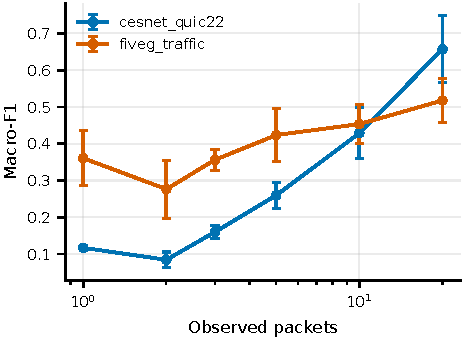
\includegraphics[width=\columnwidth]{figures/early_classification.pdf}
\caption{Macro-F1 against the number of observed packets, encoder frozen,
prototypes rebuilt at each budget. A deployment does not receive the whole
flow; this curve, not the full-flow number, determines whether a classifier can
sit inline. Note that the cumulative feature channels are normalised by fixed
constants rather than by the observation window's total, so truncating the
sequence is exactly equal to observing fewer packets --- normalising by the
total would let the value at packet~1 depend on packets not yet seen and
silently inflate the left of this curve.}
\label{fig:early}
\end{figure}

Figure~\ref{fig:early} shows accuracy against the observation budget. Twenty
packets recover most of the full-flow result; below five, the task is close to
undetermined.

\subsection{Cross-dataset transfer}

\begin{figure}[t]
\centering
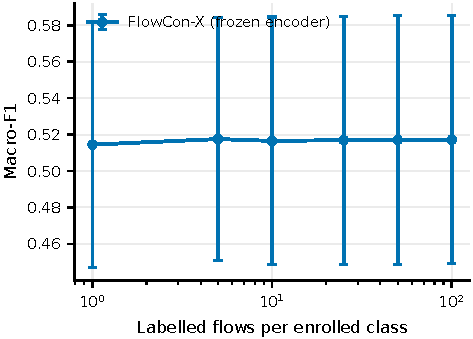
\includegraphics[width=\columnwidth]{figures/enrollment_curve.pdf}
\caption{Enrollment curves with the encoder frozen: macro-F1 against the number
of labelled flows per enrolled class, with the spread over repeated draws.
Within a corpus the curve is flat, because the prototypes are already correct.
The informative version of this experiment is across corpora
(\S\ref{sec:negative}), where they are not.}
\label{fig:enrollment}
\end{figure}

One encoder trained on one corpus and applied frozen to the other, over the
three classes the two taxonomies share, transfers poorly zero-shot: 0.246 and
0.286 macro-F1, at or below a trivial predictor, with only
\texttt{streaming} carrying across at all. Five labelled flows per class
recover 0.676 in the CESNET~$\rightarrow$~5G direction, which is 91\% of the
value reached at a hundred. \S\ref{sec:negative} discusses what that means for
the enrollment claim, and Figure~\ref{fig:enrollment} shows the within-corpus
curve it corrects.

\subsection{Cost}

% Generated by scripts/make_paper_assets.py. Do not edit by hand.
\begin{table}[t]
\centering
\small
\begin{tabular}{lccccccc}
\toprule
Method & p50 (ms) & p95 (ms) & p99 (ms) & Flows/s & Params & Size (MB) & New class \\
\midrule
FlowCon-X & 6.05 & 6.79 & 8.17 & 7863 & 1\,406\,342 & 5.7 & $k$ fwd passes \\
DeepPacket-style CNN & \textsc{todo} & \textsc{todo} & \textsc{todo} & \textsc{todo} & 270\,918 & 1.1 & fine-tune \\
FS-Net & \textsc{todo} & \textsc{todo} & \textsc{todo} & \textsc{todo} & 634\,258 & 2.5 & fine-tune \\
Bi-LSTM + attention & \textsc{todo} & \textsc{todo} & \textsc{todo} & \textsc{todo} & 573\,331 & 2.3 & fine-tune \\
Flow-statistics MLP & \textsc{todo} & \textsc{todo} & \textsc{todo} & \textsc{todo} & 73\,234 & 0.3 & fine-tune \\
\bottomrule
\end{tabular}
\caption{Deployment cost, measured on identical hardware. Latency percentiles are end-to-end -- stored record in, decision out, including feature construction -- at batch size 1, not a mean of the forward pass alone. The last column is the cost of adding one new application: a prototype update needs $k$ forward passes, a softmax classifier needs a fine-tuning run.}
\label{tab:cost}
\end{table}


End-to-end latency is measured from stored record to decision, including
parsing and feature construction, at batch size one: 6.85\,ms median, 8.70\,ms
at the 95th and 10.34\,ms at the 99th percentile, 7{,}301 flows per second
batched. We report percentiles
rather than a mean because the tail decides whether a classifier can sit
inline, and we include feature extraction because excluding it measures
something a deployment never experiences.
